\documentclass[11pt,hyperref={bookmarks=false}]{beamer}
\usetheme{Warsaw}
%\usetheme{Madrid}
%\usecolortheme{beaver}
\usefonttheme{professionalfonts}
% \usepackage[usenames,dvipsnames]{pstricks}
 \usepackage{wallpaper}
 \usepackage{epsfig}
\definecolor{UniBlue}{RGB}{157,34,53}
\setbeamercolor{block title}{bg=UniBlue!70,fg=black}

\usepackage{psfrag,graphicx}
\usepackage{amsmath,amsfonts}
%\usepackage{lscape}
\usepackage{array,epsfig}
\usepackage{amsfonts}
\usepackage{amssymb}
\usepackage{amsxtra}
\usepackage{amsthm}
\usepackage{makecell}
\usepackage[skip=0pt, belowskip=-10pt]{caption}
%\usepackage{subcaption}
\usepackage{float}
\usepackage{multirow}
%\usepackage{makecell}
\usepackage{adjustbox}
\usepackage{ulem}
\usepackage{threeparttable}

\usepackage{booktabs}
%\usepackage{subfigure}
%\usepackage{eso-pic}
%\usepackage{transparent}
%\usepackage{graphicx}
%\usepackage{tikz}
%\usepackage{longtable}
\newtheorem{df}{Definition}
\newtheorem{lm}{Lemma}
\newtheorem{prp}{Proposition}
\newtheorem{sprf}{Sketch of Proof}
\newtheorem{prf}{Proof}
\newtheorem{conjecture}{Conjecture}
\newtheorem{suffc}{Sufficient Condition}
\setbeameroption{hide notes}
\newcommand{\threelinebracer}{$\left. \begin{array}{c} \\ \\ \\ \end{array} \right\rbrace$}
\newcommand{\threelinebracel}{$\left. \begin{array}{c} \\ \\ \\ \end{array} \right\lbrace$}
\newcommand{\twolinebracer}{$\left. \begin{array}{c} \\ \\ \end{array} \right\rbrace$}
\newcommand{\twolinebracel}{$\left. \begin{array}{c} \\ \\ \end{array} \right\lbrace$}
\newcommand{\bd}{\partial}

\usepackage{pgf}  
%\logo{\pgfputat{\pgfxy(-1.2,-0.2)}{\pgfbox[center,base]{\includegraphics[height=12pt, keepaspectratio]{UA_Logo_Horizontal.eps}}} }

%\usebackgroundtemplate
%{
  %  \node[opacity=0.3, at=(current page.south east),anchor=south east,inner sep=0pt] 
    %\includegraphics[width=\paperwidth,height=20pt]{UA_Logo_Horizontal.eps}%
%}

\linespread{1}
\usepackage{parskip}
%\setlength{\itemsep}{1em} 
%\addtolength{\parskip}{5pt}
\DeclareMathSizes{12}{10}{8}{6}
%  \begin{itemize}}{\end{itemize}}
% Separate slides by \begin{frame} and \end{frame}.
\title[Willingness-to-pay for Warnings]{Willingness-to-pay for Warnings}
\author[A. Gaduh, P. McGee and A. Ugarov]{A. Gaduh, P. McGee and A. Ugarov}
\institute[]{}
\date{\today}

\newcommand\BackgroundPic{%
\put(0,0){%
\parbox[b][\paperheight]{\paperwidth}{%
\vfill
\centering
%\includegraphics[width=\paperwidth,height=\paperheight,%keepaspectratio]{sancho.png}%
\vfill
}}}


\begin{document}
%\AddToShipoutPicture*{\BackgroundPic}

\begin{frame}
\titlepage
\end{frame}

%%%%%%%%%%%%%%%%%%%%%%%%%%%%%%%%%%%%%%%%%%%%%%%%%%%%%%%%%%%%%%%%%%%%%%%%%%%%%%%%%%%%%%%%%%%%%%%%
%%%%%%%%%%%%%%%%%%%%%%%%%%%%%%%%%%%%%%%%%%%%%%%%%%%%%%%%%%%%%%%%%%%%%%%%%%%%%%%%%%%%%%%%%%%%%%%%




\begin{frame}
\frametitle{Willingness to Pay for Warnings}
\framesubtitle{Research Question}
\begin{itemize}
	\item How much do people value alerts (signals) about potential preventable threats?
	\item How do signal's probabilistic characteristics affect the willingness-to-pay for it and the welfare gains from using it?
	\item Applications:
	\begin{itemize}
		\item Natural disaster warnings (tornados, floods, earthquakes)
		\item Medical tests for treatable conditions
		\item Investing in research on likelihood of catastrophic events (rogue AI, global warming, pandemics)
	\end{itemize}
	\item Note: most real-life applications provide little practice with using the signal
\end{itemize}
\end{frame}


\begin{frame}
\frametitle{Overview of the Experiment}
\framesubtitle{Willingness to pay (WTP) for signals}
\begin{itemize}
	\item An insurance experiment:
		\begin{itemize}
			\item Two states of the world: bad ($\omega=1$) and good ($\omega=0$)
			\item Probability of a bad state is $P (\omega=1) = \pi$
			\item Bad state $\implies$ loss of \$$L$
			\item A perfectly protective insurance can be purchased for \$$c$
		\end{itemize}
	\item Subject can purchase a signal $s$ before purchasing the insurance:
		\begin{itemize}
			\item A signal is characterized by its true-positive ($P(s=1|\omega=1)$) and true-negative rates ($P(s=0|\omega=0)$) 
		\end{itemize}
\end{itemize}

\vspace{1em}
\begin{block}{Research objective}
	How do signal characteristics affect the WTP for the signal?
\end{block}
\end{frame}



\begin{frame}
\frametitle{WTP for Signals}
\framesubtitle{Theory}

\begin{itemize}
	\item Theoretically, what should be the WTP for a signal?
	\item If bad states are a priori rare ($\pi L<<c$) $\implies$ never protect without a signal
	\item The theoretical WTP $b$ for an expected utility maximizer given a signal $s$ is a solution $b^*$ to the following:
	\[
	\small
	\begin{split}
		P(s=1) &u(Y_0-b^*-c) + \pi P(s=0|\omega=1)u(Y_0-b^*-L)+\\ 
		&+(1-\pi)P(s=0|\omega=0)u(Y_0-b^*) =\\
		&=(1-\pi)u(Y_0)+\pi u(Y_0-L)
	\end{split}
	\]
	\normalsize
	\item A risk-neutral agent would therefore pay:
		\[b^*=\pi(1-P(s=0|\omega=1))L-P(s=1)c\]
\end{itemize}
\end{frame}


\begin{frame}
\frametitle{Experiment Basics}
\begin{enumerate}
\item A box with 20 white and black balls (black ball=bad state)
\item Assumptions:
\begin{itemize}
\item Protection cost is \$5
\item Loss without protection is \$20
\item Cost-loss ratio is $c/L=5/20=0.25$
\end{itemize}
\item Signal is an unreliable hint about the ball color
\item Vary the prior probability of bad state and the signal's information structure
\end{enumerate}
\end{frame}

\begin{frame}
\frametitle{Hypotheses}
\begin{itemize}
        \item Subjects' relative weights on FP and FN rates are consistent with the risk-neutral EU model:
       \item More specifically:
       $$b^*=\alpha \underbrace{P(s=1|\omega=0)(1-\pi)c}_{ \textrm{FP Costs} } +\beta \underbrace{P(s=0|\omega=1) \pi L}_{ \textrm{FN Costs} } + Z+\epsilon$$
       $$ H0:\alpha=\beta$$
       \item If true - signal designers just need to balance the potential costs of FP and FN events (FP and FN costs)
       \item Additionally: we need to understand the sources of deviation if they exist (beliefs, risk preferences, information preferences)
       \item Presentation of probabilistic information can change beliefs
\end{itemize}
\end{frame}


\begin{frame}
\frametitle{Experiment Progression}
\begin{enumerate}
\item \textbf{Blind Protection Game:} Protection response conditional on prior probability
\item \textbf{Informed Protection Game:} Protection response conditional on prior probability and signal
\item \textbf{Belief Elicitation:} Subjects beliefs about the bad state's probability conditional on prior and signal
\item \textbf{WTP Elicitation:} Willingness-to-pay for each signal
\end{enumerate}
\end{frame}


\begin{frame}
\frametitle{Main Results}
\begin{itemize}
\item Subjects underweight both the prior probability and the signal (consistent with all the tasks using signals)
\item Subjects's WTP underreact to false positive rates for low priors and overreact for high probabilities
\item The opposite is true for false negative rates
\item Incorrect belief formation is largely responsible for the bias
\end{itemize}
\end{frame}



\begin{frame}
\frametitle{Experimental Design}
\begin{itemize}
\item xxxx
\end{itemize}
\end{frame}


\begin{frame}
\frametitle{Sample}
\begin{itemize}
\item xxxx
\end{itemize}
\end{frame}


\begin{frame}
\frametitle{Overview/Our Data Makes Sense Graphs}
\begin{itemize}
\item xxxx
\end{itemize}
\end{frame}



\begin{frame}
\frametitle{WTP Discrepancy}
\begin{figure}[h]
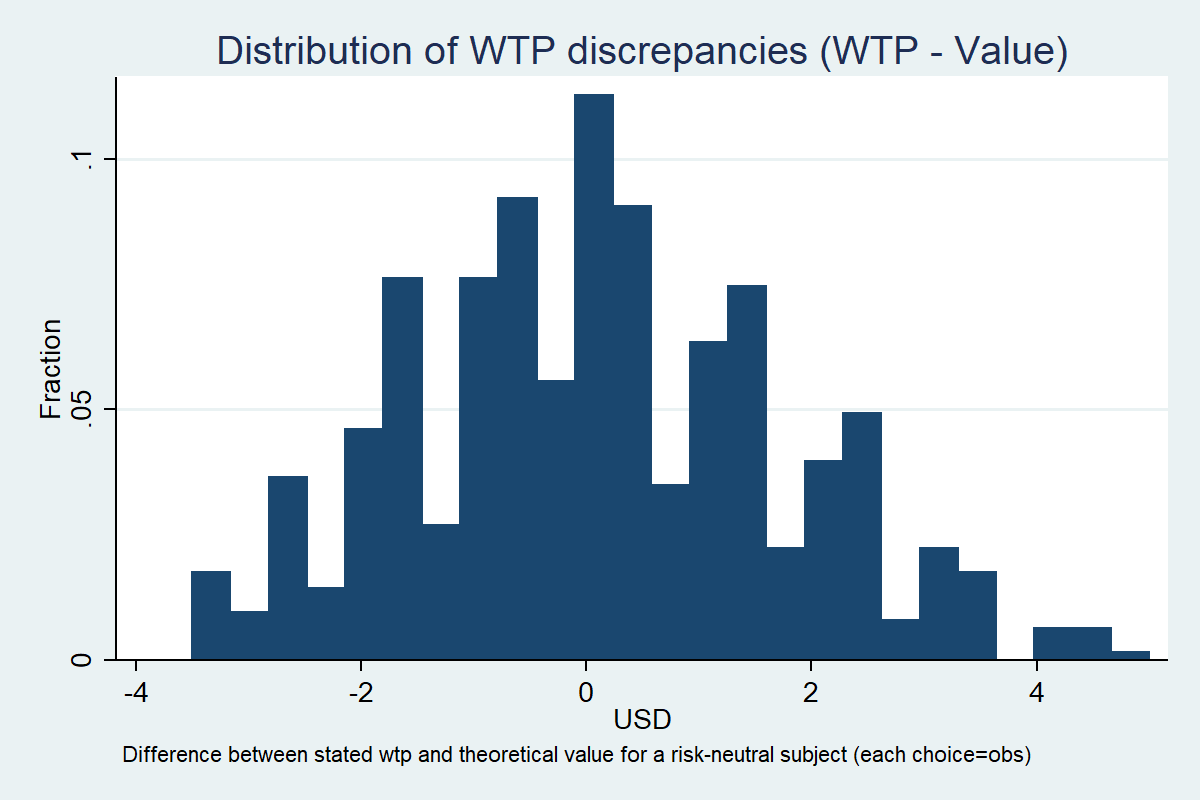
\includegraphics[scale=0.25]{Graphs/hist_WTP_discr1.png}
\end{figure}
\end{frame}






\begin{frame}
\frametitle{WTP Big Picture}
\begin{itemize}
\item Subjects overpay for signals with both FP and FN (low-quality signals)
\item WTP for other signal types is not significantly different from the risk-neutral model
\end{itemize}

\small
\begin{table}[H]\centering \begin{tabular}{cccc} \hline \hline
\textbf{False-positive}&\textbf{False-negative}&\textbf{Mean WTP discrepancy}& \textbf{P($=0$)}\\ \hline
No&No&-0.106&0.433\\
No&Yes&0.143&0.250\\
Yes&No&0.081&0.502\\
Yes&Yes&0.492&0.000\\
\hline \end{tabular} \end{table}

\end{frame}




\begin{frame}
\frametitle{WTP Sensitivity}
\begin{itemize}
\item Subjects underreact to both false-positive and false-negative rates
\item Underweighting is not explained by risk aversion or belief accuracy
\item No evidence of \textbf{relative} underweighting of FP or FN signals on average
\item Large heterogeneity with respect to priors!
\end{itemize}
\end{frame}


\begin{frame}
\frametitle{WTP Sensitivity Table}
\begin{figure}[h]
\includegraphics[scale=0.55]{table_WTP_OLS.png}
\end{figure}

\end{frame}


\begin{frame}
\frametitle{WTP for signals: Heterogeneity with respect to priors}
\begin{itemize}
\item Relative overweighting of FN costs for low priors; overweighting of FP costs for high priors
\item Note: this already accounts for higher frequency of FP and FN events; what happens is that subjects underestimate the importance in FP and FN rates
\end{itemize}
\footnotesize
\begin{table}[htbp]\centering
\def\sym#1{\ifmmode^{#1}\else\(^{#1}\)\fi}
\caption{WTP - Value of Information, by prior}
\begin{tabular}{l*{4}{c}}
\hline\hline
                &\multicolumn{1}{c}{(1)}&\multicolumn{1}{c}{(2)}&\multicolumn{1}{c}{(3)}&\multicolumn{1}{c}{(4)}\\
                &\multicolumn{1}{c}{0.1}&\multicolumn{1}{c}{0.2}&\multicolumn{1}{c}{0.3}&\multicolumn{1}{c}{0.5}\\
\hline
FP costs        &     .437\sym{***}&     .576\sym{***}&   -.0356         &    -.346         \\
                &    (0.1)         &    (0.2)         &    (0.2)         &    (0.3)         \\
FN costs        &    -.645\sym{***}&     .196         &     .254\sym{***}&     .379\sym{***}\\
                &    (0.2)         &    (0.1)         &    (0.1)         &    (0.1)         \\
Constant        &     .467\sym{***}&    -.713\sym{***}&    -.877\sym{***}&     .677\sym{***}\\
                &    (0.1)         &    (0.1)         &    (0.1)         &    (0.2)         \\
\hline
Observations    &      159         &      153         &      159         &      153         \\
Adjusted \(R^{2}\)&     0.63         &     0.49         &     0.40         &     0.48         \\
\hline\hline
\multicolumn{5}{l}{\footnotesize Standard errors in parentheses}\\
\multicolumn{5}{l}{\footnotesize Subject fixed effects are included.}\\
\multicolumn{5}{l}{\footnotesize \sym{*} \(p<0.10\), \sym{**} \(p<0.05\), \sym{***} \(p<0.01\)}\\
\end{tabular}
\end{table}

\end{frame}


\begin{frame}
\frametitle{WTP for signals: Heterogeneity with respect to priors}
\begin{itemize}
\item In terms of pure FP and FN rates, there is more sensitivity for higher priors
\item But little differentiation between FP and FN - all sensitivities increase despite the model predicting that FN is more important for higher priors
\end{itemize}
\scriptsize
\begin{table}[htbp]\centering
\def\sym#1{\ifmmode^{#1}\else\(^{#1}\)\fi}
\caption{WTP for Information (Tobit, by prior)}
\begin{tabular}{l*{4}{c}}
\hline\hline
                &\multicolumn{1}{c}{(1)}&\multicolumn{1}{c}{(2)}&\multicolumn{1}{c}{(3)}&\multicolumn{1}{c}{(4)}\\
                &\multicolumn{1}{c}{0.1}&\multicolumn{1}{c}{0.2}&\multicolumn{1}{c}{0.3}&\multicolumn{1}{c}{0.5}\\
\hline
model           &                  &                  &                  &                  \\
FP rate         &    -2.81\sym{**} &    -2.08\sym{**} &    -4.35\sym{***}&    -3.25\sym{**} \\
                &    (1.1)         &    (1.0)         &    (1.0)         &    (1.3)         \\
FN rate         &    -2.45\sym{**} &    -2.73\sym{***}&    -3.67\sym{***}&    -3.65\sym{***}\\
                &    (1.1)         &    (1.0)         &    (1.0)         &    (1.3)         \\
Constant        &     1.72\sym{***}&     2.33\sym{***}&     2.63\sym{***}&     3.32\sym{***}\\
                &    (0.2)         &    (0.2)         &    (0.2)         &    (0.3)         \\
\hline
sigma           &                  &                  &                  &                  \\
Constant        &     1.86\sym{***}&      1.7\sym{***}&     1.77\sym{***}&     2.16\sym{***}\\
                &    (0.1)         &    (0.1)         &    (0.1)         &    (0.2)         \\
\hline
Observations    &      162         &      153         &      162         &      153         \\
Adjusted \(R^{2}\)&                  &                  &                  &                  \\
\hline\hline
\multicolumn{5}{l}{\footnotesize Standard errors in parentheses}\\
\multicolumn{5}{l}{\footnotesize \sym{*} \(p<0.10\), \sym{**} \(p<0.05\), \sym{***} \(p<0.01\)}\\
\end{tabular}
\end{table}

\end{frame}




\begin{frame}
\frametitle{WTP Heterogeneity Explanations}
\begin{itemize}
\item Excluded explanations:
\begin{itemize}
\item Risk preferences: both risk-averse and risk-loving subjects demonstrate the same pattern (?) 
\item Anchoring: subjects do not take into account the change in priors
\item Probability weighting
\end{itemize}
\item Non-excluded explanations: 
\begin{itemize}
\item Many subjects poorly differentiate between FP and FN signals: dishonest gremlins lower their WTP regardless of type
\item Value of non-instrumental information: certainty effects, paying for belief changes
\end{itemize}
\end{itemize}
\end{frame}


\begin{frame}
\frametitle{FP or FN? It's confusing}
\begin{itemize}
\item Both IP and BE responses demonstrate overreacting to FP rates with white signals and to FN rates with black signals
\item We confirm this pattern in the regression analysis (see further slides)
\item Many subjects report in their explanations that they try to play safe when there any dishonest gremlins!
\end{itemize}
\end{frame}



\begin{frame}
\frametitle{Belief Errors}
\begin{itemize}
\item Subjects overestimate the black ball chances when the signal is white
\item This includes overestimation for cases when false-positive outcomes are possible consistent with confusion observed in other tasks
\item Underestimation for black signals with false-negative events 
\end{itemize}
\footnotesize
\begin{table}[H]\centering \caption{Average Belief Error by Signal Type} \begin{tabular}{ccccc} \hline \hline
\textbf{False-positive}&\textbf{False-negative}&\textbf{Signal=Black}&\textbf{Belief error}& \textbf{P($=0$)}\\ \hline
No&No&No&0.039&0.001\\
No&No&Yes&-0.186&0.000\\
No&Yes&No&0.142&0.000\\
No&Yes&Yes&-0.337&0.000\\
Yes&No&No&0.118&0.000\\
Yes&No&Yes&0.173&0.000\\
Yes&Yes&No&0.245&0.000\\
Yes&Yes&Yes&0.192&0.000\\
\hline \end{tabular} \end{table}

\end{frame}



\begin{frame}
\frametitle{Belief Errors}
\begin{itemize}
\item The presence of both FP and FN rates creates overestimation of black ball chances with white signals
\item With black signals: FP rates lead to overestimation, FN - to underestimation
\end{itemize}
\footnotesize
\begin{table}[htbp]\centering
\def\sym#1{\ifmmode^{#1}\else\(^{#1}\)\fi}
\caption{Belief Elicitation: When Mistakes Happen}
\begin{tabular}{l*{3}{c}}
\hline\hline
                &\multicolumn{1}{c}{(1)}&\multicolumn{1}{c}{(2)}&\multicolumn{1}{c}{(3)}\\
                &\multicolumn{1}{c}{All}&\multicolumn{1}{c}{S=White}&\multicolumn{1}{c}{S=Black}\\
\hline
FP rate         &    0.600\sym{***}&    0.292\sym{***}&    0.908\sym{***}\\
                &  (0.057)         &  (0.063)         &  (0.102)         \\
FN rate         &    0.011         &    0.273\sym{***}&   -0.251\sym{***}\\
                &  (0.053)         &  (0.061)         &  (0.084)         \\
A92             &   -0.018\sym{*}  &   -0.145\sym{***}&    0.108\sym{***}\\
                &  (0.009)         &  (0.010)         &  (0.016)         \\
B113            &   -0.088\sym{***}&   -0.372\sym{***}&    0.196\sym{***}\\
                &  (0.009)         &  (0.010)         &  (0.016)         \\
B139            &    0.140\sym{***}&   -0.190\sym{***}&    0.470\sym{***}\\
                &  (0.000)         &  (0.000)         &  (0.000)         \\
B61             &   -0.170\sym{***}&   -0.177\sym{***}&   -0.163\sym{***}\\
                &  (0.000)         &  (0.000)         &  (0.000)         \\
B87             &    0.084\sym{***}&   -0.305\sym{***}&    0.473\sym{***}\\
                &  (0.001)         &  (0.001)         &  (0.002)         \\
C108            &    0.104\sym{***}&   -0.299\sym{***}&    0.506\sym{***}\\
                &  (0.001)         &  (0.001)         &  (0.002)         \\
C134            &    0.006         &   -0.205\sym{***}&    0.217\sym{***}\\
                &  (0.009)         &  (0.010)         &  (0.016)         \\
C56             &    0.005         &   -0.326\sym{***}&    0.337\sym{***}\\
                &  (0.009)         &  (0.010)         &  (0.016)         \\
C82             &    0.056\sym{***}&   -0.248\sym{***}&    0.360\sym{***}\\
                &  (0.000)         &  (0.000)         &  (0.000)         \\
D103            &    0.123\sym{***}&   -0.207\sym{***}&    0.453\sym{***}\\
                &  (0.000)         &  (0.000)         &  (0.000)         \\
D129            &    0.086\sym{***}&   -0.326\sym{***}&    0.498\sym{***}\\
                &  (0.001)         &  (0.001)         &  (0.002)         \\
D51             &    0.070\sym{***}&   -0.241\sym{***}&    0.381\sym{***}\\
                &  (0.001)         &  (0.001)         &  (0.002)         \\
D77             &    0.024\sym{**} &   -0.289\sym{***}&    0.337\sym{***}\\
                &  (0.009)         &  (0.010)         &  (0.016)         \\
E124            &    0.084\sym{***}&   -0.350\sym{***}&    0.518\sym{***}\\
                &  (0.000)         &  (0.000)         &  (0.000)         \\
E150            &    0.125\sym{***}&   -0.312\sym{***}&    0.561\sym{***}\\
                &  (0.001)         &  (0.001)         &  (0.002)         \\
E46             &    0.052\sym{***}&   -0.340\sym{***}&    0.443\sym{***}\\
                &  (0.000)         &  (0.000)         &  (0.000)         \\
E72             &    0.071\sym{***}&   -0.265\sym{***}&    0.406\sym{***}\\
                &  (0.001)         &  (0.001)         &  (0.002)         \\
E98             &    0.142\sym{***}&   -0.116\sym{***}&    0.400\sym{***}\\
                &  (0.009)         &  (0.010)         &  (0.016)         \\
F119            &    0.003         &   -0.314\sym{***}&    0.319\sym{***}\\
                &  (0.009)         &  (0.010)         &  (0.016)         \\
F41             &    0.080\sym{***}&   -0.307\sym{***}&    0.467\sym{***}\\
                &  (0.009)         &  (0.010)         &  (0.016)         \\
F67             &    0.123\sym{***}&   -0.334\sym{***}&    0.580\sym{***}\\
                &  (0.000)         &  (0.000)         &  (0.000)         \\
F93             &    0.093\sym{***}&   -0.305\sym{***}&    0.490\sym{***}\\
                &  (0.001)         &  (0.001)         &  (0.002)         \\
G114            &    0.122\sym{***}&   -0.284\sym{***}&    0.528\sym{***}\\
                &  (0.001)         &  (0.001)         &  (0.002)         \\
G140            &   -0.023\sym{**} &   -0.065\sym{***}&    0.018         \\
                &  (0.009)         &  (0.010)         &  (0.016)         \\
G62             &   -0.002         &   -0.425\sym{***}&    0.420\sym{***}\\
                &  (0.009)         &  (0.010)         &  (0.016)         \\
G88             &    0.039\sym{***}&   -0.315\sym{***}&    0.393\sym{***}\\
                &  (0.000)         &  (0.000)         &  (0.000)         \\
H109            &    0.122\sym{***}&   -0.287\sym{***}&    0.532\sym{***}\\
                &  (0.000)         &  (0.000)         &  (0.000)         \\
H135            &    0.070\sym{***}&   -0.341\sym{***}&    0.481\sym{***}\\
                &  (0.001)         &  (0.001)         &  (0.002)         \\
H57             &   -0.022\sym{***}&   -0.301\sym{***}&    0.256\sym{***}\\
                &  (0.001)         &  (0.001)         &  (0.002)         \\
H83             &    0.082\sym{***}&   -0.280\sym{***}&    0.444\sym{***}\\
                &  (0.009)         &  (0.010)         &  (0.016)         \\
I104            &   -0.003         &   -0.193\sym{***}&    0.187\sym{***}\\
                &  (0.009)         &  (0.010)         &  (0.016)         \\
I130            &    0.090\sym{***}&   -0.247\sym{***}&    0.427\sym{***}\\
                &  (0.000)         &  (0.000)         &  (0.000)         \\
I52             &    0.010\sym{***}&   -0.215\sym{***}&    0.235\sym{***}\\
                &  (0.000)         &  (0.000)         &  (0.000)         \\
I78             &    0.127\sym{***}&   -0.277\sym{***}&    0.531\sym{***}\\
                &  (0.001)         &  (0.001)         &  (0.002)         \\
J125            &    0.037\sym{***}&   -0.047\sym{***}&    0.121\sym{***}\\
                &  (0.009)         &  (0.010)         &  (0.016)         \\
J151            &   -0.043\sym{***}&   -0.157\sym{***}&    0.070\sym{***}\\
                &  (0.000)         &  (0.000)         &  (0.000)         \\
J47             &    0.073\sym{***}&   -0.264\sym{***}&    0.409\sym{***}\\
                &  (0.009)         &  (0.010)         &  (0.016)         \\
J73             &    0.162\sym{***}&   -0.212\sym{***}&    0.537\sym{***}\\
                &  (0.000)         &  (0.000)         &  (0.000)         \\
J99             &    0.041\sym{***}&   -0.235\sym{***}&    0.316\sym{***}\\
                &  (0.001)         &  (0.001)         &  (0.002)         \\
K120            &    0.127\sym{***}&   -0.277\sym{***}&    0.531\sym{***}\\
                &  (0.001)         &  (0.001)         &  (0.002)         \\
K42             &    0.004\sym{***}&   -0.324\sym{***}&    0.331\sym{***}\\
                &  (0.001)         &  (0.001)         &  (0.002)         \\
K68             &    0.035\sym{***}&   -0.213\sym{***}&    0.283\sym{***}\\
                &  (0.009)         &  (0.010)         &  (0.016)         \\
K94             &    0.056\sym{***}&   -0.298\sym{***}&    0.410\sym{***}\\
                &  (0.000)         &  (0.000)         &  (0.000)         \\
L115            &    0.081\sym{***}&   -0.152\sym{***}&    0.313\sym{***}\\
                &  (0.000)         &  (0.000)         &  (0.000)         \\
L141            &   -0.056\sym{***}&   -0.201\sym{***}&    0.090\sym{***}\\
                &  (0.001)         &  (0.001)         &  (0.002)         \\
L63             &    0.056\sym{***}&   -0.320\sym{***}&    0.431\sym{***}\\
                &  (0.001)         &  (0.001)         &  (0.002)         \\
L89             &    0.089\sym{***}&   -0.135\sym{***}&    0.314\sym{***}\\
                &  (0.009)         &  (0.010)         &  (0.016)         \\
M110            &    0.008         &   -0.033\sym{***}&    0.048\sym{***}\\
                &  (0.009)         &  (0.010)         &  (0.016)         \\
M136            &   -0.057\sym{***}&   -0.232\sym{***}&    0.118\sym{***}\\
                &  (0.000)         &  (0.000)         &  (0.000)         \\
M58             &   -0.094\sym{***}&   -0.382\sym{***}&    0.193\sym{***}\\
                &  (0.000)         &  (0.000)         &  (0.000)         \\
M84             &   -0.196\sym{***}&   -0.190\sym{***}&   -0.202\sym{***}\\
                &  (0.001)         &  (0.001)         &  (0.002)         \\
N105            &   -0.048\sym{***}&   -0.328\sym{***}&    0.231\sym{***}\\
                &  (0.001)         &  (0.001)         &  (0.002)         \\
N131            &   -0.019\sym{**} &   -0.409\sym{***}&    0.371\sym{***}\\
                &  (0.009)         &  (0.010)         &  (0.016)         \\
N53             &    0.039\sym{***}&   -0.414\sym{***}&    0.492\sym{***}\\
                &  (0.009)         &  (0.010)         &  (0.016)         \\
N79             &    0.078\sym{***}&   -0.375\sym{***}&    0.532\sym{***}\\
                &  (0.000)         &  (0.000)         &  (0.000)         \\
O100            &   -0.111\sym{***}&   -0.348\sym{***}&    0.127\sym{***}\\
                &  (0.000)         &  (0.000)         &  (0.000)         \\
O126            &    0.066\sym{***}&   -0.347\sym{***}&    0.478\sym{***}\\
                &  (0.001)         &  (0.001)         &  (0.002)         \\
O48             &   -0.206\sym{***}&   -0.200\sym{***}&   -0.212\sym{***}\\
                &  (0.001)         &  (0.001)         &  (0.002)         \\
O74             &    0.059\sym{***}&   -0.313\sym{***}&    0.430\sym{***}\\
                &  (0.009)         &  (0.010)         &  (0.016)         \\
P121            &    0.115\sym{***}&   -0.250\sym{***}&    0.480\sym{***}\\
                &  (0.000)         &  (0.000)         &  (0.000)         \\
P43             &    0.108\sym{***}&   -0.207\sym{***}&    0.423\sym{***}\\
                &  (0.000)         &  (0.000)         &  (0.000)         \\
P69             &   -0.272\sym{***}&   -0.251\sym{***}&   -0.294\sym{***}\\
                &  (0.001)         &  (0.001)         &  (0.002)         \\
P95             &    0.073\sym{***}&   -0.297\sym{***}&    0.442\sym{***}\\
                &  (0.009)         &  (0.010)         &  (0.016)         \\
Q116            &   -0.004         &   -0.423\sym{***}&    0.415\sym{***}\\
                &  (0.009)         &  (0.010)         &  (0.016)         \\
Q142            &    0.056\sym{***}&   -0.248\sym{***}&    0.360\sym{***}\\
                &  (0.000)         &  (0.000)         &  (0.000)         \\
Q64             &    0.102\sym{***}&   -0.248\sym{***}&    0.452\sym{***}\\
                &  (0.000)         &  (0.000)         &  (0.000)         \\
Q90             &   -0.181\sym{***}&   -0.259\sym{***}&   -0.104\sym{***}\\
                &  (0.001)         &  (0.001)         &  (0.002)         \\
R111            &   -0.089\sym{***}&   -0.068\sym{***}&   -0.110\sym{***}\\
                &  (0.001)         &  (0.001)         &  (0.002)         \\
R137            &   -0.190\sym{***}&   -0.294\sym{***}&   -0.086\sym{***}\\
                &  (0.009)         &  (0.010)         &  (0.016)         \\
R59             &    0.080\sym{***}&   -0.322\sym{***}&    0.482\sym{***}\\
                &  (0.009)         &  (0.010)         &  (0.016)         \\
R85             &    0.120\sym{***}&   -0.269\sym{***}&    0.508\sym{***}\\
                &  (0.000)         &  (0.000)         &  (0.000)         \\
S106            &   -0.344\sym{***}&   -0.348\sym{***}&   -0.340\sym{***}\\
                &  (0.000)         &  (0.000)         &  (0.000)         \\
S132            &    0.121\sym{***}&   -0.319\sym{***}&    0.561\sym{***}\\
                &  (0.001)         &  (0.001)         &  (0.002)         \\
S54             &    0.119\sym{***}&   -0.312\sym{***}&    0.550\sym{***}\\
                &  (0.001)         &  (0.001)         &  (0.002)         \\
S80             &    0.029\sym{***}&   -0.283\sym{***}&    0.342\sym{***}\\
                &  (0.009)         &  (0.010)         &  (0.016)         \\
T101            &   -0.025\sym{***}&   -0.349\sym{***}&    0.299\sym{***}\\
                &  (0.009)         &  (0.010)         &  (0.016)         \\
T127            &    0.102\sym{***}&   -0.324\sym{***}&    0.528\sym{***}\\
                &  (0.000)         &  (0.000)         &  (0.000)         \\
T49             &   -0.127\sym{***}&   -0.224\sym{***}&   -0.030\sym{***}\\
                &  (0.000)         &  (0.000)         &  (0.000)         \\
T75             &    0.048\sym{***}&   -0.343\sym{***}&    0.440\sym{***}\\
                &  (0.001)         &  (0.001)         &  (0.002)         \\
U122            &    0.022\sym{**} &   -0.375\sym{***}&    0.418\sym{***}\\
                &  (0.009)         &  (0.010)         &  (0.016)         \\
U44             &    0.021\sym{**} &   -0.408\sym{***}&    0.450\sym{***}\\
                &  (0.009)         &  (0.010)         &  (0.016)         \\
U70             &    0.089\sym{***}&   -0.290\sym{***}&    0.468\sym{***}\\
                &  (0.000)         &  (0.000)         &  (0.000)         \\
U96             &   -0.035\sym{***}&   -0.195\sym{***}&    0.125\sym{***}\\
                &  (0.001)         &  (0.001)         &  (0.002)         \\
V117            &    0.072\sym{***}&   -0.338\sym{***}&    0.481\sym{***}\\
                &  (0.001)         &  (0.001)         &  (0.002)         \\
V65             &    0.137\sym{***}&   -0.110\sym{***}&    0.384\sym{***}\\
                &  (0.009)         &  (0.010)         &  (0.016)         \\
V91             &    0.107\sym{***}&   -0.249\sym{***}&    0.462\sym{***}\\
                &  (0.000)         &  (0.000)         &  (0.000)         \\
W112            &    0.101\sym{***}&   -0.225\sym{***}&    0.427\sym{***}\\
                &  (0.000)         &  (0.000)         &  (0.000)         \\
W138            &   -0.088\sym{***}&   -0.232\sym{***}&    0.056\sym{***}\\
                &  (0.001)         &  (0.001)         &  (0.002)         \\
W60             &   -0.038\sym{***}&   -0.257\sym{***}&    0.181\sym{***}\\
                &  (0.001)         &  (0.001)         &  (0.002)         \\
W86             &    0.008         &   -0.351\sym{***}&    0.367\sym{***}\\
                &  (0.009)         &  (0.010)         &  (0.016)         \\
X107            &   -0.097\sym{***}&   -0.380\sym{***}&    0.187\sym{***}\\
                &  (0.009)         &  (0.010)         &  (0.016)         \\
X133            &   -0.227\sym{***}&   -0.232\sym{***}&   -0.222\sym{***}\\
                &  (0.000)         &  (0.000)         &  (0.000)         \\
X55             &   -0.177\sym{***}&   -0.190\sym{***}&   -0.163\sym{***}\\
                &  (0.000)         &  (0.000)         &  (0.000)         \\
X81             &   -0.089\sym{***}&   -0.218\sym{***}&    0.040\sym{***}\\
                &  (0.001)         &  (0.001)         &  (0.002)         \\
Y102            &    0.105\sym{***}&   -0.302\sym{***}&    0.511\sym{***}\\
                &  (0.001)         &  (0.001)         &  (0.002)         \\
Y128            &   -0.020\sym{**} &   -0.068\sym{***}&    0.028\sym{*}  \\
                &  (0.009)         &  (0.010)         &  (0.016)         \\
Y50             &   -0.055\sym{***}&   -0.368\sym{***}&    0.258\sym{***}\\
                &  (0.009)         &  (0.010)         &  (0.016)         \\
Y76             &    0.093\sym{***}&   -0.248\sym{***}&    0.435\sym{***}\\
                &  (0.000)         &  (0.000)         &  (0.000)         \\
Z123            &   -0.043\sym{***}&   -0.351\sym{***}&    0.265\sym{***}\\
                &  (0.001)         &  (0.001)         &  (0.002)         \\
Z149            &    0.141\sym{***}&    0.118\sym{***}&    0.164\sym{***}\\
                &  (0.009)         &  (0.010)         &  (0.016)         \\
Z45             &   -0.157\sym{***}&   -0.276\sym{***}&   -0.039\sym{***}\\
                &  (0.001)         &  (0.001)         &  (0.002)         \\
Z71             &    0.031\sym{***}&   -0.399\sym{***}&    0.461\sym{***}\\
                &  (0.009)         &  (0.010)         &  (0.016)         \\
Z97             &    0.066\sym{***}&    0.035\sym{***}&    0.097\sym{***}\\
                &  (0.000)         &  (0.000)         &  (0.000)         \\
Constant        &   -0.078\sym{***}&    0.314\sym{***}&   -0.470\sym{***}\\
                &  (0.007)         &  (0.009)         &  (0.013)         \\
\hline
Observations    &     1248         &      624         &      624         \\
Adjusted \(R^{2}\)&    0.146         &    0.415         &    0.521         \\
\hline\hline
\multicolumn{4}{l}{\footnotesize Standard errors in parentheses}\\
\multicolumn{4}{l}{\footnotesize Dep. variable: reported belief - posterior probability}\\
\multicolumn{4}{l}{\footnotesize \sym{*} \(p<0.10\), \sym{**} \(p<0.05\), \sym{***} \(p<0.01\)}\\
\end{tabular}
\end{table}

\end{frame}




\begin{frame}
\frametitle{Informed Protection (Big Picture)}
\begin{itemize}
\item Overprotecting with white signals when either false-positives or false-negatives are possible
\item Underprotecting in response to black signals with false-negatives
\item For an EU-maximizer, false-positives should not affect neither beliefs nor protection decision $\implies$ this violation signals confusion
\end{itemize}
\scriptsize


\begin{table}[H]\centering 

\adjustbox{max width=\textwidth}{
	\begin{threeparttable}
	\begin{tabular}{cccccccc} \hline \hline
	\multirow{4}{6ex}{\centering \textbf{Row}}
			&\multicolumn{3}{c}{\centering \textbf{Signal Characteristics}} 
			& \multirow{3}{10ex}{\centering \textbf{Posterior}} & \multirow{3}{10ex}{\centering \textbf{Share Protect}} 
			& \multirow{3}{10ex}{\centering \textbf{Share Optimal}} 
			& \multirow{3}{13ex}{\centering \textbf{P-val $(H_0: ShProt=ShOptimal)$}} \\ 
			\cmidrule(lr){2-4}
		&\multirow{2}{10ex}{\centering \textbf{Signal}} & \multirow{2}{12ex}{\centering \textbf{False Positive}} 
			& \multirow{2}{10ex}{\centering \textbf{False Negative}} 
		\\
		\\
		&(1) & (2) & (3) & (4) & (5) & (6) & (7) \\
		\hline
			(1)&White&No&No&0.000&0.067&0.000&0.000\\
(2)&White&No&Yes&0.100&0.333&0.000&0.000\\
(3)&White&Yes&No&0.000&0.130&0.000&0.000\\
(4)&White&Yes&Yes&0.131&0.564&0.121&0.000\\
(5)&Black&No&No&1.000&0.846&1.000&0.000\\
(6)&Black&No&Yes&1.000&0.841&1.000&0.000\\
(7)&Black&Yes&No&0.550&0.833&0.870&0.355\\
(8)&Black&Yes&Yes&0.483&0.886&0.871&0.685\\

			\\
		\hline\hline 
	\end{tabular} 
					
	\end{threeparttable}
	}
\end{table}
\end{frame}


\begin{frame}
\frametitle{Informed Protect: Comments on the Baseline Regressions}
\begin{itemize}
\item Both FP and FN rates increase the likelihood to protect when the signal is white
\item No significant effect when the signal is black
\item Less sensitivity to FP rate and more sensitivity to FN rate when the prior is high ($\geq 0.2$)
\item Overall pretty poor differentiation between FP and FN rates
\end{itemize}
\end{frame}


\begin{frame}
\frametitle{Informed Protection: Linear Probability Model}
\scriptsize
\begin{table}[htbp]\centering
\def\sym#1{\ifmmode^{#1}\else\(^{#1}\)\fi}
\begin{tabular}{l*{6}{c}}
\hline\hline
                &\multicolumn{1}{c}{(1)}&\multicolumn{1}{c}{(2)}&\multicolumn{1}{c}{(3)}&\multicolumn{1}{c}{(4)}&\multicolumn{1}{c}{(5)}&\multicolumn{1}{c}{(6)}\\
                &\multicolumn{1}{c}{All}&\multicolumn{1}{c}{S=White}&\multicolumn{1}{c}{S=Black}&\multicolumn{1}{c}{All}&\multicolumn{1}{c}{S=White}&\multicolumn{1}{c}{W=Black}\\
\hline
FP rate         &     .284\sym{***}&     .496\sym{***}&    .0725         &     .259\sym{**} &     .613\sym{***}&   -.0949         \\
                &    (2.9)         &    (3.8)         &    (0.5)         &    (2.2)         &    (4.3)         &   (-0.5)         \\
FN rate         &     .596\sym{***}&     1.21\sym{***}&   -.0213         &     .322\sym{***}&       .7\sym{***}&   -.0564         \\
                &    (7.2)         &    (8.9)         &   (-0.2)         &    (3.0)         &    (4.0)         &   (-0.3)         \\
p$>$0.2         &     .119\sym{***}&     .138\sym{***}&    .0994\sym{***}&    .0475\sym{**} &    .0438         &    .0512         \\
                &    (6.7)         &    (5.6)         &    (3.7)         &    (2.0)         &    (1.3)         &    (1.4)         \\
FP rate x (p$>$0.2)&                  &                  &                  &    .0508         &    -.233         &     .335\sym{*}  \\
                &                  &                  &                  &    (0.4)         &   (-1.3)         &    (1.7)         \\
FN rate x (p$>$0.2)&                  &                  &                  &     .548\sym{***}&     1.03\sym{***}&    .0703         \\
                &                  &                  &                  &    (4.0)         &    (4.4)         &    (0.4)         \\
Constant        &     .759\sym{***}&      .57\sym{***}&     .948\sym{***}&     .794\sym{***}&     .617\sym{***}&     .972\sym{***}\\
                &   (47.1)         &   (24.3)         &   (43.4)         &   (43.0)         &   (23.9)         &   (37.1)         \\
Subject FE      &      Yes         &      Yes         &      Yes         &      Yes         &      Yes         &      Yes         \\
\hline
Observations    &     1248         &      624         &      624         &     1248         &      624         &      624         \\
Adjusted \(R^{2}\)&     0.08         &     0.41         &     0.27         &     0.09         &     0.44         &     0.27         \\
\hline\hline
\multicolumn{7}{l}{\footnotesize \textit{t} statistics in parentheses}\\
\multicolumn{7}{l}{\footnotesize Errors are clustered by subject}\\
\multicolumn{7}{l}{\footnotesize \sym{*} \(p<0.10\), \sym{**} \(p<0.05\), \sym{***} \(p<0.01\)}\\
\end{tabular}
\end{table}

\end{frame}



\begin{frame}
\frametitle{Informed Protection: Controlling for Beliefs}
\begin{itemize}
\item If we add flexible controls of posteriors, we can still see this extra-sensitivity to FP and FN rates 
\item $\implies$ sensitivity cannot be explained by risk preferences
\item Controlling for reported beliefs removes the large portion of unexplained sensitivity to FP and FN rates!
\item Beliefs do not explain informed protection completely $\implies$ subjects change beliefs between tasks $\implies$ all of the extra-sensitivity might follow from incorrect beliefs
\end{itemize}
\end{frame}



\begin{frame}
\frametitle{Informed Protection: Flexible Controls for Posteriors/Beliefs, LPM}
\scriptsize
{
\def\sym#1{\ifmmode^{#1}\else\(^{#1}\)\fi}
\begin{tabular}{l*{4}{c}}
\hline\hline
                &\multicolumn{1}{c}{(1)}&\multicolumn{1}{c}{(2)}&\multicolumn{1}{c}{(3)}&\multicolumn{1}{c}{(4)}\\
                &\multicolumn{1}{c}{}&\multicolumn{1}{c}{}&\multicolumn{1}{c}{}&\multicolumn{1}{c}{}\\
\hline
FP rate x (S=White)&     .434\sym{***}&     .508\sym{***}&     .235\sym{*}  &     .293\sym{**} \\
                &    (3.2)         &    (3.4)         &    (1.8)         &    (2.0)         \\
FN rate x (S=White)&      .43\sym{*}  &     .412         &    .0513         &    .0366         \\
                &    (1.8)         &    (1.7)         &    (0.2)         &    (0.1)         \\
FP rate x (S=Black)&    -.128         &   -.0328         &    -.187         &    -.114         \\
                &   (-0.3)         &   (-0.1)         &   (-0.4)         &   (-0.2)         \\
FN rate x (S=Black)&    .0434         &    -.067         &  .000394         &   -.0827         \\
                &    (0.4)         &   (-0.4)         &    (0.0)         &   (-0.5)         \\
S=Black         &     .342\sym{*}  &     .382\sym{*}  &     .196         &     .225         \\
                &    (2.0)         &    (1.8)         &    (1.1)         &    (1.1)         \\
p$>$0.2         &    .0504\sym{**} &    .0434\sym{*}  &    .0299         &    .0251         \\
                &    (2.5)         &    (1.9)         &    (1.5)         &    (1.1)         \\
FP rate x (p$>$0.2)&                  &    -.131         &                  &    -.101         \\
                &                  &   (-0.8)         &                  &   (-0.6)         \\
FN rate x (p$>$0.2)&                  &     .221         &                  &     .165         \\
                &                  &    (1.3)         &                  &    (1.1)         \\
Subject FE      &      Yes         &      Yes         &      Yes         &      Yes         \\
Posterior       &      Yes         &      Yes         &      Yes         &      Yes         \\
Beliefs         &       No         &       No         &      Yes         &      Yes         \\
\hline
Observations    &     1248         &     1248         &     1248         &     1248         \\
Adjusted \(R^{2}\)&     0.53         &     0.53         &     0.55         &     0.55         \\
\hline\hline
\multicolumn{5}{l}{\footnotesize \textit{t} statistics in parentheses}\\
\multicolumn{5}{l}{\footnotesize \sym{*} \(p<0.10\), \sym{**} \(p<0.05\), \sym{***} \(p<0.01\)}\\
\end{tabular}
}

\end{frame}



\begin{frame}
\frametitle{WTP Non-Instrumental Information}
\begin{itemize}
\item Subjects can put value on signals even when the signals are useless for decision-making (Eliaz and Schotter, 2010; Neumann et al, 2012)
\item We account for certainty effect ($P(S=W)(1-\mu_W)+P(S=B)\mu_B$ - expected probability that the signal is correct) and for the expected belief change (difference in subject's belief btw white and black signals for each information structure)
\item We find some evidence of preferences for non-instrumental information, but cannot differentiate these findings from incorrect belief formation
\item (Insert Table WTP regression with certainty, belief change and prior heterogeneity.)
\end{itemize}
\end{frame}


\begin{frame}
\frametitle{Strategy Heterogeneity}
\begin{itemize}
\item Some subjects indicate that they take into account only the proportion of lying gremlings regardless of their type
\item Do subjects indeed use diverse heuristics to make informed protection and WTP choices in the experiment? Does it explain the biases we observe in the data?
\item Estimate a latent class logit model to identify and explore the role of strategy heterogeneity in informed protection responses
\item The model postulates that the probability to observe a sequence of choices $y_{ij1},y_{ij2},..y_{ijR}$ for subject $i$ is:
$$P(y_{ir})=\prod_{r=1}^R \prod_{j=1}^2\left({\exp(\beta_c X_{ijr})\over \sum_{k=0}^1 \exp(\beta_c X_{ikr})} \right)^y_{ijr}$$
\item (Latent class analysis for OLS regressions with WTP?)
\item (Also why not a linear probability model for informed protection? We have no confidence that the model is not misspecified.)
\end{itemize}
\end{frame}


\begin{frame}
\frametitle{Strategy Heterogeneity}
\scriptsize
\begin{tabular}{l*{4}{c}}
\hline\hline
            &class\_compar&            &            &            \\
            &   N Classes&         BIC&         AIC&AIC corrected\\
\hline
r1          &           1&    1125.514&    1112.292&    1130.514\\
r2          &           2&     1038.58&    1017.425&     1046.58\\
r3          &           3&    1029.376&    997.6436&    1041.376\\
r4          &           4&    1025.432&    983.1217&    1041.432\\
\hline\hline
\end{tabular}

\end{frame}

\begin{frame}
\frametitle{Two Classes}
\scriptsize
\begin{table}[htbp]\centering
\def\sym#1{\ifmmode^{#1}\else\(^{#1}\)\fi}
\caption{IP response by class}
\begin{tabular}{l*{2}{c}}
\hline\hline
                &\multicolumn{1}{c}{(1)}&\multicolumn{1}{c}{(2)}\\
                &\multicolumn{1}{c}{Honesty Seekers}&\multicolumn{1}{c}{Cautious Bayesians}\\
\hline
S=Black         &     .337\sym{***}&    .0245         \\
                &    (3.4)         &    (0.4)         \\
Prop. of lying gremlins&     .664\sym{***}&     .277\sym{***}\\
                &    (4.6)         &    (4.3)         \\
Posterior prob. &    -.198\sym{*}  &     .788\sym{***}\\
                &   (-1.7)         &    (4.9)         \\
\hline
N               &      138         &      486         \\
Pseudo R-squared&     .183         &     .541         \\
Log-likelihood  &    -67.2         &     -154         \\
\hline\hline
\multicolumn{3}{l}{\footnotesize \textit{t} statistics in parentheses}\\
\multicolumn{3}{l}{\footnotesize Errors are clustered by subject, average marginal treatment effects}\\
\multicolumn{3}{l}{\footnotesize \sym{*} \(p<0.10\), \sym{**} \(p<0.05\), \sym{***} \(p<0.01\)}\\
\end{tabular}
\end{table}

\end{frame}


\begin{frame}
\frametitle{Conclusion}
\begin{itemize}
\item People lack sophistication when choosing alarm systems $\implies$ overpaying for low-value signals, discounting some good systems
\item Relative to the risk-neutral decision-makers people are not cautious enough of signals with FN rates when priors are low, and overly cautious of FP rates when the priors are high 
\item Belief formation seems to explain a large part of the bias $\implies$ different presentation of signals' characteristics should help
\item At the same time, beliefs do not explain the bias completely, and some part of it can come from preferences
\item \textit{(Needs testing: more data for low priors, varying presentation order, different way to describe/present signal characteristics (!), elicit beliefs on different signal values)}
\end{itemize}
\end{frame}



\end{document}
